\documentclass[14pt]{beamer}
\usepackage[T2A]{fontenc}
\usepackage[utf8]{inputenc}
\usepackage[english]{babel}
\usepackage{amssymb,amsfonts,amsmath,mathtext}
\usepackage{cite,enumerate,float,indentfirst}
\usepackage{graphicx}
\usepackage{multicol}
\usepackage[boxed,algochapter,noline,czech]{algorithm2e}

\renewcommand{\vec}[1]{\ensuremath{\boldsymbol{#1}}}

\graphicspath{{images/}}

\usetheme{Pittsburgh}
\usecolortheme{whale}

\setbeamercolor{footline}{fg=blue}
\setbeamertemplate{footline}{
  \leavevmode%
  \hbox{%
  \begin{beamercolorbox}[wd=.333333\paperwidth,ht=2.25ex,dp=1ex,center]{}%
    Boris Kudryashov, ITMO University
  \end{beamercolorbox}%
  \begin{beamercolorbox}[wd=.333333\paperwidth,ht=2.25ex,dp=1ex,center]{}%
    St. Petersburg, 2016
  \end{beamercolorbox}%
  \begin{beamercolorbox}[wd=.333333\paperwidth,ht=2.25ex,dp=1ex,right]{}%
  Page \insertframenumber{} of \inserttotalframenumber \hspace*{2ex}
  \end{beamercolorbox}}%
  \vskip0pt%
}

\newcommand{\itemi}{\item[\checkmark]}

\title{\small{Information Theory. 3rd Chapter Slides}}
\author{\huge{
Boris Kudryashov \\
\vspace{30pt}
ITMO University
}}


\begin{document}

\maketitle

\begin{frame}
\frametitle{Agenda}
\begin{enumerate}    
% \footnotesize {
% \small{
    
\item Universal coding task
\item Useful combinatorial formulas
\item Two pass encoding
\item Enumerative coding
\item Asymptotic bounds of redundancy
\item Adaptive coding
\item Algorithm comparison

\end{enumerate}
\end{frame}

\begin{frame}
\frametitle{Universal coding task}
\begin{itemize}    
% \footnotesize {
% \small{
    
    \item  \textit{Encoding redundancy} for a model class $\Omega$ is
    \begin{equation}
    \label{redundancy}
     r_n(\Omega ) = \mathop {\sup }\limits_{ \omega \in \Omega }
    \left[ {\bar {R}_n(\omega)- H_\omega } \right].
    \end{equation}
    
    \item Coding is called \textit{Universal} if for algorithm holds
    \[
    \lim_{n\rightarrow \infty}  r_n(\Omega ) =0,
    \]
    
\end{itemize}
\end{frame}


% ----------------------Useful combinatorial formulas------------

\begin{frame}
\frametitle{Useful combinatorial formulas}
\begin{itemize}    
% \footnotesize {
\small{
    
    \item Consider sequences $\vec x = (x_1 ,...,x_n )$, where $x_i$ has one of $M_i$ values, $i = 1,...,n$. Number of different $\vec x$ is
    \begin{equation}
    \label{eq3_1} \left| {\left\{ {\vec x = (x_1 ,...,x_n ):x_i \in
    \{0,...,M_i - 1\},i = 1,...n} \right\}} \right| = \prod\limits_{i = 1}^n {M_i } .
    \end{equation}
    
    \item 
    \begin{equation}
    \label{eq3_2}
    A_M^n = M(M - 1)\times ...\times (M - n + 1)
    =\frac{M!}{(M - n)!} .
    \end{equation}
}    
\end{itemize}
\end{frame}


\begin{frame}
\frametitle{Useful combinatorial formulas}
\begin{itemize}    
% \footnotesize {
% \small{
    
    \item Number of combinations
    \begin{eqnarray}
    \label{eq3_4} C_M^n &=&\binom M n = \frac{A_M^n }{P_n }=\nonumber\\
    &=& \frac{M(M - 1)\times ...\times (M - n + 1)}{n!} =\nonumber\\
    &=& \frac{M!}{n!(M - n)!}.
    \end{eqnarray}
   
    \item Number of combinations
    \begin{equation}
    \label{eq3_5} %
    \binom n k = \left\{
    \begin{array} {cl}
    \frac {n!}{k!(n - k)!}, &\mbox{if } n\ge k\ge 0 \\
    1,       &\mbox{if } n\ge 0 \mbox{ and } k=0 \mbox{ or } k=n\\
    0,       &\mbox{if } k<0 \mbox{ or } k>n
    \end{array} \right 
    \end{equation}


\end{itemize}
\end{frame}


\begin{frame}
\frametitle{Useful combinatorial formulas}
\begin{itemize}    
% \footnotesize {
\small{

    \item binomial coefficient 
    \[
    (a + b)^n = \sum\limits_{k = 0}^n \binom n k  a^k b^{n-k}.
    \]
    
    \item Number os binary sequences of length $n$, which contain $\tau _1 $ ones and $\tau _0 = n - \tau _1 $ zeros.
    \begin{equation}
    \label{eq3_6} N(\tau _0 ,\tau _1 ) = \binom n {\tau _0}=
    \frac{n}{\tau _0 !\tau _1 !}.
    \end{equation}
    
    \item Composition of sequence $\vec x$ is vector $\vec \tau (\vec x) = (\tau _0 (\vec x),...,\tau _{M - 1} (\vec x))$, where $\tau _i (\vec x)$ denotes number of elements $x_t = i$ in sequence $\vec x = (x_1 ,...,x_n )$.
  
}
\end{itemize}
\end{frame}


\begin{frame}
\frametitle{Useful combinatorial formulas}
\begin{itemize}    
% \footnotesize {
\small{ 
    
    % \item For $M=3$
    % \[
    % N(\vec \tau) = \binom  n {\tau _0 } \binom {n - \tau _0 } {\tau _1 } = \frac{n!}{\tau _0 !(n - \tau _0 )!}\frac{(n - \tau _0 )!}{\tau _1 !(n - \tau _0 - \tau _1 )!} = \frac{n!}{\tau _0 !\tau _1 !\tau _2 !}.
    % \]
    
    \item For arbitrary $M$
    \begin{equation}
    \label{eq3_7} N(\vec \tau) = \frac{n!}{\tau _0 !...\tau _{M - 1} !}.
    \end{equation}
    
    \item Newton formula generalization
    \[
    (a_0 + ... + a_{M - 1} )^n = \sum\limits_{\vec \tau:~\tau _0 + ... + \tau _{M - 1} = n} {N(\vec \tau)\prod\limits_{i = 0}^{M - 1} {a_i^{\tau _i } } } .
    \]
}
\end{itemize}
\end{frame}


\begin{frame}
\frametitle{Useful combinatorial formulas}
\begin{itemize}    
% \footnotesize {
\small{
    
    \item Consider the following lemma:
    \begin{lemma} \label{num_comp} $n \in mathbb{N}$ can be written as sum of $M$ non-negative integer terms in $\binom  {n + M - 1} {M - 1} $ ways. 
    \end{lemma}

    \item Number of different compositions of sequence of length $n$ over $M$-size alphabet is
    \begin{equation}
    \label{eq3_8}
    N_\tau (n,M) = \binom {n + M - 1} {M - 1}
    \end{equation}
    
    \item Stirling formula
    \begin{equation}
    \label{eq3_9} \sqrt {2\pi n} n^ne^{ - n}\exp \left\{ {\frac{1}{12n + 1}} \right\} < n! < \sqrt {2\pi n} n^ne^{ - n}\exp \left\{ {\frac{1}{12n}} \right\}.
    \end{equation}  
 }   
\end{itemize}
\end{frame}


\begin{frame}
\frametitle{Useful combinatorial formulas}
\begin{itemize}    
% \footnotesize {
\small{    
    
    
    \item Consider
    \[
    N(\vec \tau) < (2\pi n)^{ - \frac{M - 1}{2}}2^{n\log n -
    \sum\limits_i {\tau _i \log \tau _i } }\left( {\prod\limits_i
    {\frac{n}{\tau _i }} } \right)^{1 / 2}\times
    \]
    \begin{equation}
    \label{eq3_10} \times \exp \left\{ {\frac{1}{12n} - \sum\limits_i
    {\frac{1}{12\tau _i + 1}} } \right\}.
    \end{equation}
    
    \item Logarithm of number of sequences with specified composition
    \begin{equation}
    \label{eq3_11} \log N(\vec \tau) < nH(\vec {\hat p}) - \frac{M -1}{2}\log (2\pi n) - \frac{1}{2}\sum\limits_i {\log (\hat {p}_i )} ,
    \end{equation}
}
\end{itemize}
\end{frame}


\begin{frame}
\frametitle{Useful combinatorial formulas}
\begin{itemize}    
% \footnotesize {
\small{
    
    \item More compact estimation
    \begin{equation}
    \label{eq3_12} \log N(\vec \tau) < nH(\vec {\hat p}) - \frac{M - 1}{2}\log (2\pi n) + \frac{1}{2}\log \frac{n}{n - M + 1}.
    \end{equation}
    
    \item Recurrent formula holds
    \begin{equation}
    \label{eq3_13} \binom {n+1} w =\binom n w+\binom n {w-1} .
    \end{equation}
    
    \item 
    \begin{equation}
    \label{eq3_14} \binom {n+1} w =\binom n w+ \binom {n-1} {w-1} + ... + \binom {n-w+1} 1.
    \end{equation}
} 
\end{itemize}
\end{frame}
    
% -----------------------Two pass encoding-------------


\begin{frame}
\frametitle{Two pass encoding}
\begin{itemize}    

% \small{

    \item {
    \footnotesize {
    \begin{equation}
    \label{ex2pass} {\texttt{
    IF{\_}WE{\_}CANNOT{\_}DO{\_}AS{\_}WE{\_}WOULD{\_}WE{\_}SHOULD{\_}DO{\_}AS{\_}WE{\_}CAN} }\\
    \end{equation}
    }
    }

    \item 
    \[
    l_2 = 6 + 6 + 12\times 2 + 5\times 3 + ... + 6 = 178.
    \]
    
    \item 
    \begin{center}
    00010000010100110111101101111.
    \end{center}

\end{itemize}
\end{frame}
    

\begin{frame}
\frametitle{Two pass encoding}
\begin{itemize}    
% \footnotesize {
% \small{    
    
    \item 
    \[
    l_1 = 29 + 8\times 15 = 149\text{~bit}.
    \]
    
    \item 
    \begin{equation}
    \label{eq3_15} l = l_1 + l_2 = 149 + 178 = 327\text{~bit}.
    \end{equation}
   
\end{itemize}
\end{frame}

\begin{frame}
\frametitle{Two pass encoding}
\begin{itemize}    
% \footnotesize {
% \small{

    \begin{table}[htbp]
    \caption{Huffman code for text (\ref{ex2pass})}
    \begin{center}
    \scalebox{0.65}{
    \begin{tabular}{|c|c|c|l|}
    \hline %
    Character &Number of & Codeword& Codeword  \\
          &iterations &   length       &  \\\hline %
    I   & 1 & 6 & 010000 \\ \hline %
    F   & 1 & 6 & 010001 \\ \hline %
    {\_}& 12& 2&  00     \\ \hline %
    W   & 5 & 3 & 100    \\ \hline %
    E   & 4 & 4 & 0101   \\ \hline %
    C   & 2 & 5 & 01001  \\ \hline %
    A   & 4 & 4 & 1010   \\ \hline %
    N   & 3 & 4 & 1011   \\ \hline %
    O   & 5 & 3 & 110    \\ \hline %
    T   & 1 & 6 & 011110 \\ \hline %
    D   & 4 & 4 & 0110   \\ \hline %
    S   & 3 & 4 & 1110   \\ \hline %
    U   & 2 & 4 & 1111   \\ \hline %
    L   & 2 & 5 & 01110  \\ \hline %
    H   & 1 & 6 & 011111 \\\hline
    \end{tabular}
    }
    \end{center}
    \label{tab2pass}
    \end{table}
    
\end{itemize}
\end{frame}



\begin{frame}
\frametitle{Two pass encoding}
\begin{itemize}    
% \footnotesize {
% \small{

    \begin{figure}[ht]
    \begin{minipage}{1.0\linewidth}
    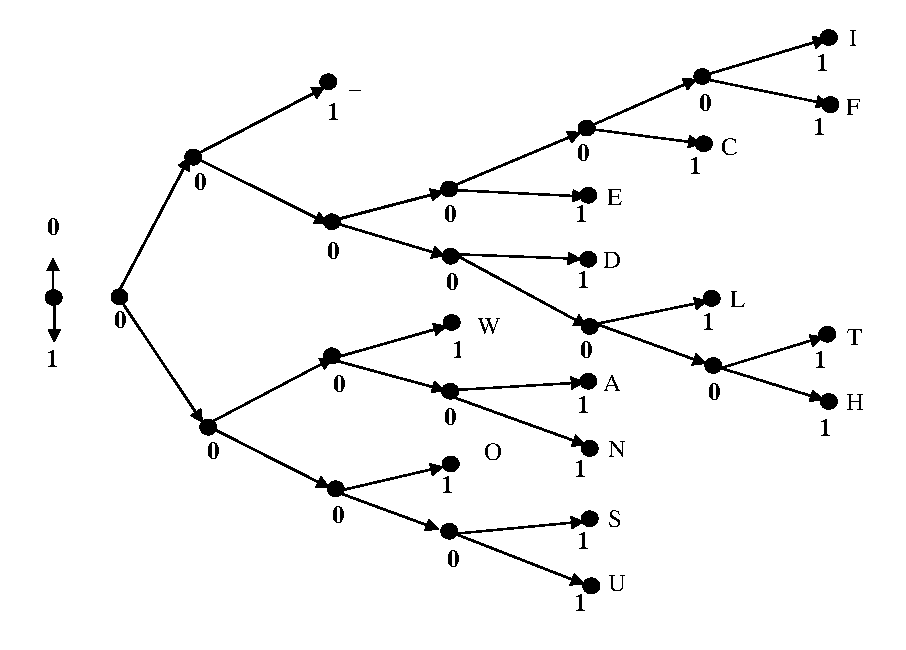
\includegraphics[width=1.0\textwidth]{fig3_1.eps}
    \caption{Huffman codetree for (\ref{ex2pass})}
    \label{HUF_tree}
    \end{minipage}
    \end{figure}
    
\end{itemize}
\end{frame}



\begin{frame}
\frametitle{Two pass encoding}
\begin{itemize}    
% \footnotesize {
% \small{
    \begin{table}[htbp]
    \label{tab2pass_reg} \caption{Regular Huffman code}
    \scalebox{0.65}{
    \begin{tabular}
    {|c|c|l|} \hline %
    Character & Codeword length & Codeword\\ \hline%
    {\_} & 2 & 00     \\ \hline %
    O    & 3 & 010    \\ \hline %
    W    & 3 & 011    \\ \hline %
    A    & 4 & 1000   \\ \hline %
    D    & 4 & 1001   \\ \hline %
    E    & 4 & 1010   \\ \hline %
    N    & 4 & 1011   \\ \hline %
    S    & 4 & 1100   \\ \hline %
    U    & 4 & 1101   \\ \hline %
    C    & 5 & 11100  \\ \hline %
    L    & 5 & 11101  \\ \hline %
    F    & 6 & 111100 \\ \hline %
    H    & 6 & 111101 \\ \hline %
    I    & 6 & 111110 \\ \hline %
    T    & 6 & 111111 \\ \hline
    \end{tabular}
    }
    \label{tab2}
    \end{table}
\end{itemize}
\end{frame}



\begin{frame}
\frametitle{Two pass encoding}
\begin{itemize}    
% \footnotesize {
% \small{

    \begin{table}[htbp]
    \caption{Number of bits for regular code tree transmitting}
    \scalebox{0.75}{
    \begin{tabular}
    {|c|c|c|c|c|}\hline %
    Level& Number of & Number of & Range of & Expenses  \\ %
        & nodes  &  leaves  $n_i $& values $n_i $&in bits \\ \hline %
    0& 1& 0& 0\ldots 1& 1 \\ \hline %
    1& 2& 0& 0\ldots 2& 2 \\ \hline %
    2& 4& 1& 0\ldots 4& 3 \\ \hline %
    3& 6& 2& 0\ldots 6& 3 \\ \hline %
    4& 8& 6& 0\ldots 8& 4 \\ \hline %
    5& 4& 2& 0\ldots 4& 3 \\ \hline %
    6& 4& 4& 0\ldots 4& 3 \\ \hline %
    Всего& \multicolumn{3}{c|}{}&19 \\ \hline %
    \end{tabular}
    }
    \label{tab_bits_for_tree}
    \end{table}
    
\end{itemize}
\end{frame}



\begin{frame}
\frametitle{Two pass encoding}
\begin{itemize}    
% \footnotesize {
% \small{
    \begin{figure}[ht]
    \begin{minipage}{1.0\linewidth}
    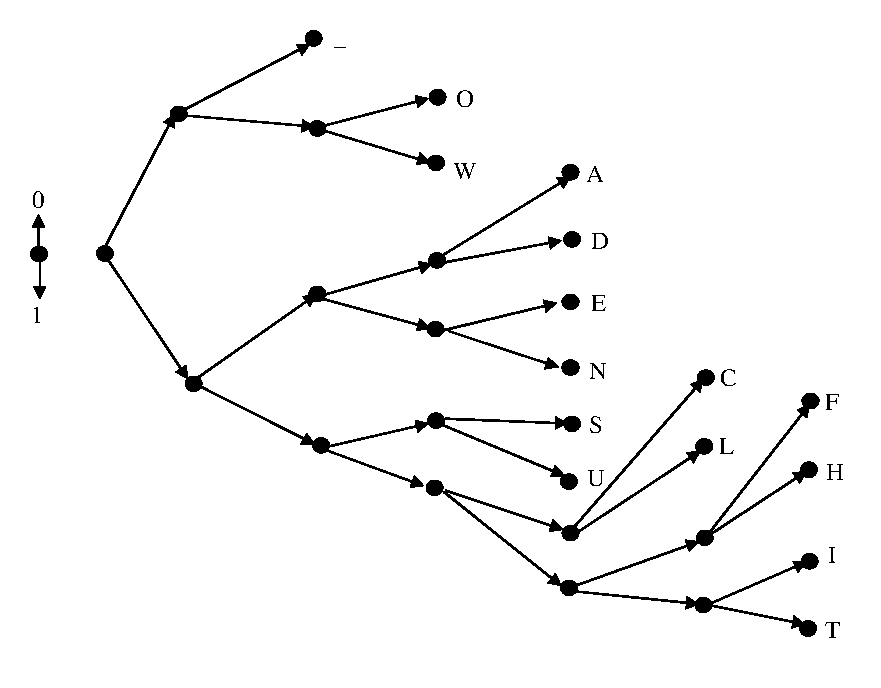
\includegraphics[width=0.85\textwidth]{fig3_2.eps}
    \caption{Codetree for regular Huffman code}
    \label{HUF_tree_reg}
    \end{minipage}
    \end{figure}
    
\end{itemize}
\end{frame}



\begin{frame}
\frametitle{Two pass encoding}
\begin{itemize}    
% \footnotesize {
% \small{

    \item Enough for transmitting information about letters that are associated with regular codetree nodes:
    \[
    \left\lceil \log \binom {256} 1 \right\rceil +%
    \left\lceil \log \binom {255} 2 \right\rceil +%
    \left\lceil \log \binom {253} 6 \right\rceil +%
    \]
    \[
    +
    \left\lceil \log \binom {247} 2 \right\rceil +%
    \left\lceil \log \binom {245} 4 \right\rceil =105 \text{~bits}
    \]
    
    \item More precise 
    \begin{equation}
    \label{eq3_16} l = 178 + 19 + 105 = 302\text{~bits} .
    \end{equation}
    
\end{itemize}
\end{frame}


\begin{frame}
\frametitle{Two pass encoding}
% \footnotesize {
% \small{

    \begin{theorem} \label{th_two_pass}
    For two pass coding with Huffman code of Discrete Memoryless Source with alphabet size $M$ and entropy $H$, average code rate satisfies
    \begin{equation}
    \label{eq3_17} \bar {R} \le H + 1 + \frac{1}{n}\left( {M\log M + 3M - 1} \right).
    \end{equation}
    \end{theorem}

\end{frame}



\begin{frame}
\frametitle{Two pass encoding}
Proof.
\begin{itemize}    

\small{

    \item
    \label{eq3_18} $l_1 (\vec x) \le 2M - 1 + M\left\lceil {\log M} \right\rceil \le M\log M + 3M - 1.$
}
\footnotesize {
    \item 
    \begin{eqnarray}
    \label{eq3_19}%
    l_2 (\vec x) &\stackrel{\rm (a)}{=}& \sum\limits_{i = 1}^n l(x_i )
    =\nonumber\\
    &\stackrel{\rm (b)}{=}& \sum\limits_{x \in X} \tau _n (x)l(x)=\nonumber\\
    &\stackrel{\rm (c)}{=}& n \sum\limits_{x \in X} \frac{\tau _n
    (x)}{n}l(x) =\nonumber\\
    &\stackrel{\rm (d)}{=}&  n\sum\limits_{x \in X} \hat {p}_n (x)l(x)= \nonumber\\
    &\stackrel{\rm (e)}{=}& n {\rm {\bf M}}_{\vec {\hat {p}}_n}\left[
    {l(x)} \right]\le \nonumber\\
    &\stackrel{\rm (f)}{\le}& n(H(\vec {\hat {p}}_n ) + 1).
    \end{eqnarray}
}

\end{itemize}
\end{frame}


\begin{frame}
\frametitle{Two pass encoding}
Proof.
\begin{itemize}    
% \footnotesize {
\small{

    \item
    \begin{eqnarray}
    \label{eq3_20}
    \bar {R}(\vec x) &=& \frac{l(\vec x)}{n} = \frac{l_1
    (\vec x) + l_2 (\vec x)}{n} \le \\
    &\le& H(\vec {\hat {p}}_n) + 1 + \frac{1}{n}\left( {M\log M + 3M -
    1} \right).
    \end{eqnarray}
    
    \item
    \begin{equation}
    \label{eq3_21} {\rm {\bf M}}\left[ {H(\vec {\hat {p}}_n} \right]
    \stackrel{\rm (a)}{\le} H\left( {{\rm {\bf M}}\left[\vec {\hat
    {p}}_n \right]} \right) \stackrel{\rm (b)}{=} H(\vec p)=H.
    \end{equation}
    
    
    \item
    \begin{equation}
    \label{eq3_22} {\rm {\bf M}}\left[ \vec {\hat {p}}_n \right] = \vec p,
    \end{equation}
    
    \item 
    \[
    {\rm {\bf M}}\left[ {\frac{\tau _n (a)}{n}} \right] = p(a),\mbox{ }a \in X.
    \]
}
\end{itemize}
\end{frame}


\begin{frame}
\frametitle{Two pass encoding}
Proof.
\begin{itemize}    
% \footnotesize {
\small{
       
    \item 
    \[
    \chi _a (x) = \left\{ {{\begin{array}{*{20}c}
     {1,\mbox{ if }x = a,} \hfill \\
     {0,\mbox{ if }x \ne a.} \hfill \\
    \end{array} }} \right.
    \]
    
    \item 
    \[
    {\rm {\bf M}}\left[ {\chi _a (x)} \right] = 1\times p(a) + 0\times
    (1 - p(a)) = p(a).
    \]
    
    \item 
    \begin{eqnarray*}
    {\rm {\bf M}}\left[ {\frac{\tau _n (a)}{n}} \right] &=&
    \frac{1}{n}{\rm {\bf M}}\left[ {\sum\limits_{i = 1}^n {\chi _a (x_i
    )} } \right] =\\
     &=& \frac{1}{n}\sum\limits_{i = 1}^n {{\rm {\bf M}}\left[ {\chi _a
    (x_i )} \right]} = \\
    &=& p(a),\mbox{ }a \in X.
    \end{eqnarray*}
}

\end{itemize}
\end{frame}


\begin{frame}
\frametitle{Two pass encoding}
\begin{itemize}    
% \footnotesize {
% \small{    
    
    \item Note, that coding redundancy satisfies
    \begin{equation}
    \label{eq3_23} r = \bar {R} - H \le 1 + \frac{K}{n},
    \end{equation}
    
    \item When using arithmetic coding, the redundancy can be achieved:
    \begin{equation}
    \label{eq3_24}
     r(n)=\frac{M-1}{n} \log n +\frac
    {K}{n},
    \end{equation}
    where $M$ alphabet size, $K$ is a constant.
    
\end{itemize}
\end{frame}

% -----------------------------Enumerative coding-------------------
\begin{frame}
\frametitle{Enumerative coding}
\begin{itemize}    
\footnotesize {
% \small{
    
    \item Codeword length 
    \begin{eqnarray}
    \label{eq3_27}
    l(\vec x) &=& l_1 (\vec x) + l_2 (\vec x) =
    \nonumber\\
    &=&\left\lceil \log N_\tau (M) \right\rceil + \left\lceil \log
    N(\vec \tau ) \right\rceil = \nonumber\\
    &=& \left\lceil \log \binom {n+M-1}{M-1} \right\rceil + \left\lceil
    \log \frac{n!}{\prod_{i = 0}^{M - 1} \tau _i (\vec x)!} \right\rceil
    \end{eqnarray}
    
    \item
    \begin{center}
    {\texttt{
    IF\_WE{\_}CANNOT{\_}DO{\_}AS{\_}WE{\_}WOULD{\_}WE{\_}SHOULD{\_}DO{\_}AS{\_}WE{\_}CAN} }\\
    \end{center}
    

    \item 
    \begin{eqnarray*}
    l_1 &=& \left\lceil \log \binom {50 + 255} {255} \right\rceil = 190
    \mbox{ bits} ,\\
    l_2 &=& \left\lceil {\log \left( {\frac{50!}{12!5!^24!^33!^22!^3}}
    \right)} \right\rceil = 150 \mbox{ bits} .
    \end{eqnarray*}
}
\end{itemize}
\end{frame}


\begin{frame}
\frametitle{Enumerative coding}
\begin{itemize}    
\footnotesize {
% \small{     
    \item 
    $\vec { \tilde {\tau }} = (\tilde {\tau }_0 ,...,\tilde {\tau }_{M - 1} )$=(12, 5, 5, 4, 4, 4, 3, 3, 2, 2, 2, 1, 1, 1, 1, 0,\ldots ., 0).
    
    \item 
    \[
    1 \le \tilde {\tau }_0 \le n, \quad  \tilde {\tau} _{j+1} \le \tilde {\tau }_{j } , \quad j \ge 0.
    \]
    
    \item It's possible to transmit number of composition, no more than 
    \begin{equation}
    \label{eq3_28} \left \lceil \log \left( n\prod\limits_{j:\tau _j > 0} {\tau _j } \right ) \right\rceil \mbox{ bits} \end{equation}
    
    \item To transmit the composition $\vec \tau'=(1,2,3,2,3,4,241)$
    \begin{equation}
    \label{eq3_29} l_1 = \left\lceil {\log \left( {n\prod\limits_{j:\tau _j > 0} {\tau _j } } \right)} \right\rceil + \left\lceil {\log \left( {\frac{M!}{\prod\limits_j {{\tau }'_j !} }} \right)} \right\rceil = 25 + 108 = 133 \mbox{ bits}.
    \end{equation}
    
}    
\end{itemize}
\end{frame}


\begin{frame}
\frametitle{Enumerative coding}
\begin{itemize}    
% \footnotesize {
% \small{
    
    \item 
    \[
    l = l_1 + l_2 = 283 \mbox{ bits}
    \]
    
    \item 
    \begin{eqnarray*}
    l(\vec x) &=& l_1 (\vec x) + l_2 (\vec x) =\\
    &=& \left\lceil {\log N_\tau (M)} \right\rceil + \left\lceil {\log
    N(\vec \tau)} \right\rceil
    \le\\
    &\le& nH({\rm {\bf \hat {p}}}) - \frac{M - 1}{2}\log (2\pi n) -\\
    &&-\frac{1}{2}\sum\limits_i {\log (\hat {p}_i )} + (M - 1)\log (n +
    1) + 1.
    \end{eqnarray*}
    
    
\end{itemize}
\end{frame}


\begin{frame}
\frametitle{Enumerative coding}   
% \footnotesize {
% \small{

    \begin{theorem}
    \label{num_coding} For enumerate coding of discrete memoryless source with alphabet size $M$ and entropy $H$, the average code rate is.
    \begin{equation}
    \label{eq3_31} \bar {R} \le H + \frac{M - 1}{2}\frac{\log (n + 1) +
    K}{n},
    \end{equation}
    where $K$ does not depend on sequence length $n$.
    \end{theorem}
    
\end{frame}



\begin{frame}
\frametitle{Enumerative coding}
Example
% \footnotesize {

\begin{itemize}
\small{
    \item 
    Let $n=10$, $\vec \tau =(2, 5, 3)$, $\vec x  = (2 0 1 1 0 2 1 2 1 1)$.
    Probability distribution on first step $\vec \tau / n=(2/10, 5/10, 3/10)$ $G=0.3$.
    
    \item 
    Probability distribution after first step:
    $(2, 5, 2)/9=(2/9, 5/9, 2/9)$. 
    
    \item 
    After second step: $G=3/10\times 2/9$. 
    
    \item 
    After $10$ steps:
    \[
    G=\frac {3}{10}\times \frac {2}{9}\times\frac {5}{8}\times
    \frac {4}{7}\times\frac {1}{6}\times
    \frac {2}{5}\times\frac {3}{4}\times\frac {1}{3}\times
    \frac {2}{2}\times\frac {1}{1}\quad.
    \]
    
    \item
    Codeword length for this example:
    \[
    l=\lceil -\log G\rceil =\left\lceil -\log \frac{10!}{2!5!3!}\right\rceil
    \]
}
\end{itemize}
\end{frame}



\begin{frame}
\frametitle{Asymptotic bounds of redundancy}
\begin{itemize}    
% \footnotesize {
% \small{

    \item Redundancy
    \begin{equation}
    \label{redundancy1}
     r_n(\Omega ) = \mathop {\sup }\limits_{ \omega \in \Omega }
    \left[ {\bar {R}_n(\omega)- H_\omega } \right].
    \end{equation}

    \item For a given $\vec \theta$ 
    \[
    p(\vec x | \vec \theta) = \prod_{i=0}^{M-1} \theta_i ^ {\tau _i(\vec x)} ,
    \]
    where $\vec \tau (\vec x) = (\tau_0(\vec x), \dots, \tau_{M-1}(\vec x))$ composition of sequence $\vec x$.

\end{itemize}
\end{frame}



\begin{frame}
\frametitle{Asymptotic bounds of redundancy}
\begin{itemize}    
% \footnotesize {
% \small{

    \item 
    \begin{equation}
    \label{eq31_0}  r_n(\Theta ) \le  \frac{M - 1}{2}\frac{\log (n + 1)
    + K}{n},
    \end{equation}
    where $K$ does not depend on $n$.
    
    \item 
    \begin{equation}
    \label{redundancy2}
    r_n(\Theta ) = \inf \mathop {\sup }\limits_{\vec \theta \in \Theta } \left[ {\bar {R}_n(\vec \theta)- H(X|\vec \theta) } \right] ,
    \end{equation}
    where $H(X|\vec \theta)$ is entropy of $X$.
    
    
\end{itemize}
\end{frame}



\begin{frame}
\frametitle{Asymptotic bounds of redundancy}
 
% \footnotesize {
% \small{
    \begin{theorem} \label{low_bound}
    For a discrete memoryless source with alphabet size $M$, 
    with redundancy of universal code $r_n(\Theta) $ per message of length $n$ holds:
    \begin{equation}
    \label{eq31_4} r_n(\Theta) \ge \frac{M - 1}{2}\frac{\log n+C}{n} ,
    \end{equation}
    where $C$ does not depend on $n$.
    \end{theorem}
\end{frame}



\begin{frame}
\frametitle{Asymptotic bounds of redundancy}
Proof of theorem.
\begin{itemize}    
% \footnotesize {
% \small{
    \item Consider $\Theta=\{ \vec \theta \}$, $f(\vec \theta)$. Required redundancy:
    \begin{equation}
    \label{redundancy3}
     r_n(\Theta ) = \inf \mathop {\sup }\limits_{f(\vec \theta)  }
    {\rm \bf {M}}_f \left[ {\bar {R}_n(\vec \theta)- H(X|\vec \theta) }
    \right] ,
    \end{equation}

    \item
    \begin{equation}
    \label{redundancy4}
     r_n(\Theta ) \ge  \mathop {\sup }\limits_{f(\vec \theta)  }
    \inf {\rm \bf {M}}_f \left[ \bar {R}_n(\vec \theta) - H(X|\vec
    \theta) \right] ,
    \end{equation}

    \item 
    \[
    \sum\limits_{\vec x \in X^n} {2^{ - l(\vec x)} \le 1} .
    \]
    
\end{itemize}
\end{frame}



\begin{frame}
\frametitle{Asymptotic bounds of redundancy}
Proof of theorem
\begin{itemize}    
% \footnotesize {


    \item
    \[
    q(\vec x) = 2^{ - l(\vec x)},
    \]
\footnotesize{    
    \item
    \[
    - \sum_ {\vec x \in X^n} p(\vec x | \vec \theta ) \log q(\vec x)   %
    \le \bar l_n (q,\vec \theta) \le %
    - \sum_ {\vec x \in X^n} p(\vec x | \vec \theta ) \log q(\vec x)   %
    +1.
    \]
}    
    \item
    \begin{equation}
    \label{eq31_1}%
    \bar l_n (q,\vec \theta) = %
    - \sum_ {\vec x \in X^n} p(\vec x | \vec \theta ) \log q(\vec x).
    \end{equation}

\end{itemize}
\end{frame}



\begin{frame}
\frametitle{Asymptotic bounds of redundancy}
Proof of theorem
\begin{itemize}    
% \footnotesize {
% \small{

    \item 
    \begin{equation}
    \label{eq31_1a}
    \bar l_n (q) = %
    - \sum_ {\vec x \in X^n} p(\vec x ) \log q(\vec x) ,
    \end{equation}

    \item
    \begin{equation}
    \label{distrib}
     p(\vec x) = {\rm {\bf M}}_f \left[ p(\vec x\vert \vec \theta
    ) \right] = %
    \int_{\vec \theta} f(\vec \theta) p(\vec x\vert \vec \theta ) d\vec
    \theta.
    \end{equation}

\end{itemize}
\end{frame}



\begin{frame}
\frametitle{Asymptotic bounds of redundancy}
Proof of theorem
\begin{itemize}    
% \footnotesize {
\small{

    \item Minimum at right is achieved, when $p(\vec x) =q(\vec x)$. 
    \[
    - \sum_ {\vec x \in X^n} p(\vec x) \log p(\vec x) + \sum_ {\vec x
    \in X^n} p(\vec x) \log q(\vec x) = - L(p||q) \le 0
    \]


    \item
    \begin{equation}
    \label{redundancy5}
     r_n(\Theta ) \ge \frac{1}{n} \mathop {\sup }\limits_{f(\vec \theta)  } %
    {\rm \bf {M}}_f \sum_{\vec x \in X^n} p(\vec x | \vec \theta)%
    \log \frac{p(\vec x | \vec \theta)}{p(\vec x)}\quad .
    \end{equation}
}    
\end{itemize}
\end{frame}


\begin{frame}
\frametitle{Asymptotic bounds of redundancy}
Proof of theorem
\begin{itemize}    
% \footnotesize {
\small{
    
    \item Dirichlet distribution:
    \begin{equation}
    \label{FDirichlet}
    f_{\vec \lambda}(\vec \theta) = \Gamma \left
    (\sum_{i=0}^{M-1} \lambda_i \right) \prod _{i=0}^{M-1} \frac
    {\theta_i^{\lambda_i -1}}{\Gamma(\lambda_i)},
    \end{equation}
    where $\vec \lambda=(\lambda_0,...,\lambda_{M-1})$ is vector of distribution parameters, $\lambda_i \ge 0$, $i=0,...,M-1$, $\Gamma(z)$ is Gamma function.
    
    \item Gamma function:
    \[
    \Gamma(z)=\int_0^\infty t^{z-1}e^{-t}dt.
    \]
    
    \item 
    \[
    \Gamma(x)=(x-1)\Gamma(x-1), \quad
    \Gamma\left(\frac{1}{2}\right)=\sqrt{\pi}.
    \]
}
\end{itemize}
\end{frame}


\begin{frame}
\frametitle{Asymptotic bounds of redundancy}
Proof of theorem
\begin{itemize}    
% \footnotesize {
% \small{

    \item 
    \[
    \Gamma(n)=(n-1)! \quad .
    \]
    
    \item 
    \[
    \Gamma(z) \approx \sqrt{2\pi}z^{z-1/2}e^{-z}, \quad z \rightarrow \infty.
    \]
    
    \item For some $K_1$
    \begin{equation}
    \label{Gam_Stirl} \left | \log \Gamma(z) + z\log e - (z-1/2)\log z
    \right | \le K_1 .
    \end{equation}

\end{itemize}
\end{frame}


\begin{frame}
\frametitle{Asymptotic bounds of redundancy}
Proof of theorem
\begin{itemize}    
% \footnotesize {
% \small{

    \item Dirichlet integral: $\forall \alpha_i$, $i=1,...,n$ and a continuous function $f$:
    \[
    \int_{\vec x: \sum_i x_i=1}{f\left(\sum_{i=1}^n x_i\right)}%
    \prod_{i=1}^{n} x_i^{\alpha_i -1} dx_1...dx_n=
    \]
    \begin{equation}
    \label{Dirichlet}%
    =\frac{\prod_{i=1}^{n}{\Gamma(\alpha_i)}}{\Gamma{\left(\sum_{i=1}^n
    \alpha_i\right)}}%
    \int_{0}^{1}f(\tau) \tau^{\left(\sum_{i=1}^n \alpha_i\right) -1} d
    \tau .
    \end{equation}


    \item Consider parameter $\lambda_i=1/2$, $i=1,...,M$,
    \begin{equation}
    \label{FDirichlet2} f(\vec \theta)=\frac{\Gamma(M/2)}{\pi^{M/2}} \prod_{i=0}^{M-1} \theta_i^{-1/2} .
    \end{equation}

\end{itemize}
\end{frame}


\begin{frame}
\frametitle{Asymptotic bounds of redundancy}
Proof of theorem
\begin{itemize}    
% \footnotesize {
% \small{

    \item 
    \[
    p(\vec x)=\frac{\Gamma(M/2)}{\pi^{M/2}}\int_{\vec
    \theta}\prod_{i=0}^{M-1} \theta_i^{\tau_i(\vec x) -1/2} d \vec
    \theta .
    \]

    \item 
    \begin{equation}
    \label{probx} %
    p(\vec x)=\frac{\Gamma(M/2)}{\pi^{M/2}}%
    \quad \frac{\prod_{i=0}^{M-1} \Gamma (\tau_i(\vec x) + 1/2 )} %
    {\Gamma (n+M/2)} .
    \end{equation}


    \item
    \begin{equation}
    \label{logprobx} %
    -\log p(\vec x)= n H \left ( \frac {\vec \tau (\vec x)}{n} \right)%
    + \frac {M-1}{2} \log n + K(n),
    \end{equation}
    where $K(n)$ is bounded
    
\end{itemize}
\end{frame}



\begin{frame}
\frametitle{Asymptotic bounds of redundancy}

% \footnotesize {
% \small{
\begin{lemma}
For a given parameters $\theta$, the average ``empirical entropy'' $H \left ( \frac {\vec \tau (\vec x)}{n} \right)$ $\forall \theta$ is connected to it's entropy
$H_{\vec \theta}(X)$ by inequalities:
\begin{equation}
\label{lemma} -\frac {K_1}{n} \le
\sum_{\vec x } p(\vec x | \vec \theta)%
H \left ( \frac {\vec \tau (\vec x)}{n} \right)-%
H_{\vec \theta}(X) \le 0 \quad,
\end{equation}
where $K_1$ is a constant, $H_{\vec \theta}(X)=-\sum_{i=0}^{M-1} \theta_i\log \theta_i$ is entropy of the source
\end{lemma}

\end{frame}



\begin{frame}
\frametitle{Asymptotic bounds of redundancy}
Proof of Lemma
\begin{itemize}    
% \footnotesize {
% \small{

    \item
    \begin{equation}
    \label{matexp}
     \sum_{\vec x } p(\vec x | \vec \theta) \tau_i
    (\vec x)=n\theta_i \quad,
    \end{equation}
    
    \item 
    \begin{equation}
    \label{matexp2}
    \sum_{\vec x } p(\vec x | \vec \theta) \tau_i^2 (\vec x)=%
    n^2\theta_i^2+n\theta_i(1-\theta_i)\quad.
    \end{equation}

\end{itemize}
\end{frame}



\begin{frame}
\frametitle{Asymptotic bounds of redundancy}
Proof of Lemma
\footnotesize {
% \small{
    
    \begin{eqnarray*}
    & & -\sum_{\vec x } p(\vec x | \vec \theta)%
     \sum_{i=0}^{M-1}\frac { \tau_i (\vec x)}{n} \log \frac {\tau_i (\vec x)}{n}%
     +\sum_{i=0}^{M-1} \theta_i\log \theta_i=\\
    &\stackrel{\rm (a)}{=}&
    -\sum_{\vec x } p(\vec x | \vec \theta)%
     \sum_{i=0}^{M-1}\frac { \tau_i (\vec x)}{n} \log \frac {\tau_i (\vec x)}{n}%
     +\sum_{\vec x } \sum_{i=0}^{M-1}p(\vec x | \vec \theta) %
     \frac {\tau_i (\vec x)}{n}\log \theta_i =\\%
    &=&-\sum_{\vec x } p(\vec x | \vec \theta)%
     \sum_{i=0}^{M-1}\frac { \tau_i (\vec x)}{n} %
     \log \frac {\tau_i (\vec x)}{n\theta_i }\ge\\%
    &\stackrel{\rm (b)}{\ge}&
     -\log\sum_{\vec x } \sum_{i=0}^{M-1}p(\vec x | \vec \theta)%
     \frac {\tau_i^2 (\vec x)}{n^2\theta_i}=\\
    &\stackrel{\rm (c)}{=}&
    =-\log\sum_{i=0}^{M-1}\frac{n^2\theta_i^2+%
    \theta_i(1-\theta_i)}{n^2\theta_i}=\\%
    &=&-\log \left( 1+\frac{M-1}{n}\right) \ge \frac{M-1}{n} \log e.
    \end{eqnarray*}
}    
\end{frame}



\begin{frame}
\frametitle{Asymptotic bounds of redundancy}
Proof of theorem
\begin{itemize}    
% \footnotesize {
% \small{

    \item
    \[
    -\sum_{\vec x \in X^n} p(\vec x | \vec \theta)%
    \log p(\vec x | \vec \theta)=H(X^n|\vec \theta )=nH_{\vec
    \theta}(X).
    \]
    
    \item
    \[
    \sum_{\vec x \in X^n} p(\vec x | \vec \theta)%
    \log \frac{p(\vec x | \vec \theta)}{p(\vec x)}\ge%
     \frac {M-1}{2} \log n + K(n)-\frac {K_1}{n} .
    \]

\end{itemize}
\end{frame}



\begin{frame}
\frametitle{Asymptotic bounds of redundancy}
Proof of theorem
\begin{itemize}    
\footnotesize {
% \small{
    
    \item
    \begin{eqnarray*}
    -\log p(\vec x)&=&%
    -\sum_{i=0}^{M-1} \tau_i(\vec x) %
    \log \left( \tau_i(\vec x)+\frac{1}{2}\right)+\\%
    && +\left(
    n+\frac{M-1}{2} \right) \log \left( n+\frac{M}{2}
    \right)+K_2= \\
    &=&-\sum_{i=0}^{M-1} \tau_i(\vec x) %
    \log \left[ \frac{\tau_i(\vec x)}{n}\left(1+%
    \frac{1}{2\tau_i(\vec x)}\right)\right]-n\log n+\\%
    &&+\left( n+\frac{M-1}{2} \right)\log n +\\
    &&+ \left( n+\frac{M-1}{2} \right)\log \left( 1+\frac{M}{2n}
    \right)+K_2,
    \end{eqnarray*}
    
    \item
    \[
    0 \le \log(1+\epsilon) \le \epsilon \log e,
    \]
}    
\end{itemize}
\end{frame}



% ----------------------Adaptive coding--------------------------

\begin{frame}
\frametitle{Adaptive coding}
Example 1
\begin{itemize}    
% \footnotesize {

    
\footnotesize {
    \item
    \begin{center}{\texttt{
    IF{\_}WE{\_}CANNOT{\_}DO{\_}AS{\_}WE{\_}WOULD{\_}WE{\_}SHOULD{\_}DO{\_}AS{\_}WE{\_}CAN} }\\
    \end{center}
}
\small{
    \item
    \[
    G = 1 \cdot \frac{1}{256}\cdot \frac{1}{257}\cdot  \frac{1}{258}
     \cdot\frac{1}{259}\cdot\frac{1}{260}\cdot\frac{2}{261} \cdot\ldots=
    \]
    \[ =\frac{12!(5!)^2(4!)^3(3!)^2(2!)^3}{256\cdot\ldots\cdot305}.
    \]
    
    \item 
    \begin{equation}
    \label{examp_alg_1} l = \left\lceil { - \log G} \right\rceil + 1 =
    342\mbox{ bits} .
    \end{equation}


    \item
    \begin{equation}
    \label{eq3_37a} \hat {p}_n (a) = \frac{\tau _n (a) + 1/2}{n + M/2}=
    \frac{2\tau _n (a) + 1}{2n + M}.
    \end{equation}
}    
\end{itemize}
\end{frame}




\begin{frame}
\frametitle{Adaptive coding}
Example 2
\begin{itemize}    
% \footnotesize {
% \small{
    
    \item
    \[
    G = 1 \cdot \frac{1}{256}\cdot \frac{1}{258}\cdot  \frac{1}{260}
     \cdot\frac{1}{262}\cdot\frac{1}{264}\cdot\frac{3}{266} \cdot\ldots=
    \]
    \[ =\frac{23!!(9!!)^2(7!!)^3(5!!)^2(3!!)^3}{256\cdot\ldots\cdot305}.
    \]

    \item
    \[(2n - 1)!! = 1\times 3\times ...\times (2n - 1),\]\[ (2n)!! = 2\times 4\times ...\times (2n).\]

    \item 
    \begin{equation}
    \label{examp_alg_2} l = \left\lceil { - \log G} \right\rceil + 1 =
    323\mbox{ bits} .
    \end{equation}

\end{itemize}
\end{frame}



\begin{frame}
\frametitle{Adaptive coding}
\begin{itemize}    
% \footnotesize {
% \small{
    
    \item
    \[
    \hat {p}_n (a) = \frac{\tau _n (a)}{n + 1}, \quad \tau _n (a) > 0.
    \]

    \item
    \[
    \hat {p}_n (esc) = \frac{1}{n + 1},
    \]

    \item \emph{A-algorithm} formula
    \begin{equation}
    \label{eq3_38} \hat {p}_n (a) = \left\{
    \begin{array}{ll}
     \frac{\tau _n (a)}{n + 1},&  \mbox{ if }\tau _n (a) > 0;  \\
     \frac{1}{n + 1} \frac{1}{M - M_n }, & \mbox{ if }\tau _n (a) = 0, \\
    \end{array}  \right.
    \end{equation}    
    
\end{itemize}
\end{frame}




\begin{frame}
\frametitle{Adaptive coding}
\begin{itemize}    
% \footnotesize {
% \small{


    \item {
    \footnotesize {
    \begin{center}{\texttt{
    IF{\_}WE{\_}CANNOT{\_}DO{\_}AS{\_}WE{\_}WOULD{\_}WE{\_}SHOULD{\_}DO{\_}AS{\_}WE{\_}CAN} }\\
    \end{center}    
    }
    }

    \item 
    \[
    G = 1 \cdot \frac{1}{2} \cdot \frac{1}{256} \cdot \frac{1}{3} \cdot \frac{1}{255} \ldots
    \]

    \item
    \[
    G = \frac{11!(4!)^2(3!)^3(2!)^2}{50!} \cdot \frac{1}{256 \cdot 255 \cdot ... \cdot 242}.
    \]

    \begin{equation}
    \label{examp_alg_a} l = \left\lceil { - \log G} \right\rceil + 1 = 291\mbox{ bits}.
    \end{equation}

\end{itemize}
\end{frame}


\begin{frame}
\frametitle{Adaptive coding}
\begin{itemize}    
\footnotesize {
% \small{
    \item for a  $\vec x = (x_1 ,...,x_n )$ with composition $(\tau _1 ,...,\tau _M )$
    \begin{eqnarray*}
    \label{eq3_39}%
     G &=& \frac{\prod\limits_{i = 1}^{M_n } {(\tau _i -
    1)!} }{n!} \cdot \frac{(M - M_n )!}{M!} =\\
    &=&\frac{\prod\limits_{i = 1}^{M_n } {\tau _i !} }{n!} \cdot
    \frac{(M - M_n )!}{M!\prod\limits_{i = 1}^{M_n } {\tau _i } } \ge\\
    &\ge& \frac{\prod\limits_{i = 1}^{M_n } {\tau _i !} }{n!}M^{ - M}(n
    + 1)^{ - M}.
    \end{eqnarray*}
}
\end{itemize}
\end{frame}


\begin{frame}
\frametitle{Adaptive coding}  
% \footnotesize {
% \small{
    \begin{theorem} 
    For adaptive arithmetic coding of discrete memoryless source with alphabet size size $M$ and entropy $H$, average code rate satisfies
    \begin{equation}
    \label{eq3_40} \bar {R} \le H + \frac{M}{2}\frac{\log (n + 1) + K}{n},
    \end{equation}
    \noindent where $K$ does not depend on $n$. 
    \end{theorem}

\end{frame}


\begin{frame}
\frametitle{Adaptive coding}
Example 4. D-algorithm
\begin{itemize}    
% \footnotesize {
% \small{

    \item  
    \begin{equation}
    \label{eq3_41} \hat {p}_n (a) = \left\{ {{\begin{array}{*{20}c}
     {\frac{\tau _n (a) - 1 / 2}{n},\mbox{ if }\tau _n (a) > 0;} \hfill \\
     {\frac{M_n }{2n}\frac{1}{M - M_n },\mbox{ if }\tau _n (a) = 0.} \hfill \\
    \end{array} }} \right.
    \end{equation}


    \item 
    \[
    G = 1 \cdot \frac{1}{2} \cdot \frac{1}{256} \cdot \frac{2}{4} \cdot
    \frac{1}{255} \cdot \frac{3}{6} \cdot \frac{1}{254}\frac{4}{8} \cdot
    \frac{1}{253}\frac{1}{10} \cdot \frac{5}{12} \cdot \frac{1}{252}...
    \]

\end{itemize}
\end{frame}


\begin{frame}
\frametitle{Adaptive coding}
Example 4. D-algorithm
\begin{itemize}    
% \footnotesize {
\small{
    \item 
    \[
    (2\times 4\times \ldots \times 100)\times (256\times 255\times
    \ldots \times 242).
    \]

    \item{ 
\footnotesize { 
    \[
    G = \frac{(2\times 12 - 3)!!((2\times 5 - 3)!!)^2((2\times 4 -
    3)!!)^3((2\times 3 - 3)!!)^2}{100!!} \times 
    \]
}    
    \[
    \times\frac{14!}{256 \cdot 255 \cdot ... \cdot 242}.
    \]
    }
    
    \item 
    \[
    l = \left\lceil { - \log G} \right\rceil + 1 = 283 \quad \mbox{bits}.
    \]
}
\end{itemize}
\end{frame}



% ----------------------Algorithm comparison----------------------

\begin{frame}
\frametitle{Algorithm comparison}
\begin{itemize}    
% \footnotesize {
% \small{
    
\footnotesize {
 
    \begin{table}[htbp]
    \caption{Universal coding algorithm comparison}
    \begin{center}
    \begin{tabular}
    {|c|c|c|c|}  \hline %
    Algorithm & Number of  & Asymptotic &   codeword length  \\ %
              & traverses  & redundancy &   for text (\ref{ex2pass})    \\%
    \hline %
    2-traverse  & 2& $1 + K_1 / n$& 302 \\%
    coding, &  &  &  \\ %
    Huffman code &  &  &  \\ \hline%
    Enumerative & 2& $\frac{M\log n + K_3 }{2n}$& 283 \\ %
    coding      &  &  &  \\\hline %
     Adaptive & 1& $\frac{M\log n + K_4 }{2n}$& 291 \\%
     coding (A) &  &  &   \\\hline %
    Adaptive  & 1& $\frac{M\log n + K_5 }{2n}$&283 \\%
    coding (D) &  &  &  \\\hline
    \end{tabular}
    \label{tab3_6} \end{center}
    \end{table}
}    
    
\end{itemize}
\end{frame}

% \item Universal coding task
% \item Useful combinatorial formulas
% \item Two pass encoding
% \item Enumerative coding
% \item Asymptotic bounds of redundancy
% \item Adaptive coding
% \item Algorithm comparison


\end{document}